\documentclass[conference]{IEEEtran}
\IEEEoverridecommandlockouts
% The preceding line is only needed to identify funding in the first footnote. If that is unneeded, please comment it out.
%Template version as of 6/27/2024

\usepackage{cite}
\usepackage{amsmath,amssymb,amsfonts}
\usepackage{algorithmic}
\usepackage{graphicx}
\usepackage{textcomp}
\usepackage{xcolor}
\def\BibTeX{{\rm B\kern-.05em{\sc i\kern-.025em b}\kern-.08em
T\kern-.1667em\lower.7ex\hbox{E}\kern-.125emX}}
\begin{document}

\title{Detecção de células fotovoltaicas defeituosas a partir de imagens de
    eletroluminescência usando redes neurais convolucionais\\
    \thanks{Universidade Federal da Bahia.}
}

\author{\IEEEauthorblockN{1\textsuperscript{st} Brenda Silva de Alencar}
    \IEEEauthorblockA{\textit{Universidade Federal da Bahia (UFBA)} \\
        Salvador, Brasil \\
        brenda.s1602@outlook.com}
}

\maketitle

\begin{abstract}
    This document is a model and instructions for \LaTeX.
    This and the IEEEtran.cls file define the components of your paper [title,
            text, heads, etc.]. *CRITICAL: Do Not Use Symbols, Special
    Characters,
    Footnotes,
    or Math in Paper Title or Abstract.
\end{abstract}

\begin{IEEEkeywords}
    component, formatting, style, styling, insert.
\end{IEEEkeywords}

\section{Introduction}
A energia fotovoltaica representa 19\% da matriz elétrica brasileira, de
acordo com a Associação Brasileira de Energia Solar Fotovoltaica (Absolar)
\cite{absolar2024}. A eficiência de sistemas de energia solar é comumente
afetada pela presença de defeitos nas células fotovoltaicas, como fissuras,
áreas inativas, e \textit{gridlines}. Sendo assim, a inspeção dos módulos
é imprescindível para obter-se um maior aproveitamento dos ativos.

O ensaio de eletroluminescência em módulos fotovoltaicos tem sido amplamente
utilizado como ferramenta na detecção de
defeitos. Durante o ensaio, o módulo examinado é colocado em ambiente escuro e
submetido à uma corrente elétrica direta, com valor semelhante à sua corrente
de curto circuito nominal.  Em seguida, capturam-se imagens do módulo
utilizando uma câmera com sensor de infravermelho capaz de capturar a radiação,
normalmente na faixa de 800 a 1150 nm, emitida pelas células
\cite{Frazao20177}. Este método não-destrutivo é eficaz em detectar anomalias
que não são reveladas na inspeção visual. Entretanto, neste processo,
é necessário que centenas de imagens sejam revisadas por um técnico, o que
compromete significativamente a eficiência da inspeção de um grande volume de
módulos, como em plantas de energia solar e em linhas de produção em fábricas
de módulos fotovoltaicos.

Desde a expansão das técnicas de aprendizado de máquina, o uso dessas
tecnologias têm se tornado cada vez mais comum na detecção de defeitos em
células fotovoltaicas. A grande quantidade de dados gerados em um ensaio de
eletroluminescência pode ser processada por algoritmos de aprendizado de
máquina, que são capazes de identificar padrões em imagens e classificar as
células fotovoltaicas como defeituosas ou não. \cite{Pratt2023} propôs
dois modelos
para determinar a probabilidade de uma célula estar danificada, o primeiro
utiliza a arquitetura
Máquina de Vetores de Suporte (SVM) e o segundo usa uma Rede Neural
Convolucional (CNN). O primeiro modelo atingiu uma acurácia média de 82.44\%,
enquanto o segundo atingiu 88.42\%. Em trabalhos mais recentes
(\cite{Pratt2023},\cite{Pratt2021}), são
utilizados modelos de segmentação de imagem baseados em aprendizagem profundo
de máquina para classificar defeitos e características encontradas das células
fotovoltaicas.\cite{Pratt2023} avaliou a eficácia de x modelos treinados para
classificar
24 tipos de defeitos e características em células fotovoltaicas.
Dentre os modelos analisados, o DeepLabv3+ obtive o melhor
desempenho, obtendo um recall de 86\% na identificação de fissuras.

Este trabalho apresenta um modelo para determinar a
possibilidade da célula estar danificada utilizando uma arquitetura de rede
neural convolucional (CNN). CNNs são amplamente utilizadas em tarefas de
classificação e visão computacional, devido a sua capacidade de extrair padrões
em imagens [REF IBM]. Esta arquitetura possui três tipos de camadas:
convolucional, \textit{pooling} e totalmente conectada. A camada convolucional
é o alicerce principal de uma CNN, onde a imagem é processada por filtros
(\textit{kernels}) que
extraem características da imagem. A camada de \textit{pooling} é utilizada
entre as camadas convolucionais a fim reduz o número de parâmetros da rede. E
por fim a camada totalmente conectada, que é responsável por realizar a
classificação final. O modelo proposto contêm 3 camadas convolucionais, com 32,
32 e 128 filtros, respectivamente. Entre essas camadas, são intercaladas
camadas de
\textit{pooling} e \textit{dropout}, para evitar o \textit{overfitting} do
modelo.

O treinamento do modelo foi realizado com imagens de
eletroluminescência de células fotovoltaicas disponibilizadas por
\cite{Deitsch2021}.

\section{Desenvolvimento}

Fig.\ref{fig:metodologia} sintetiza a metodologia nas etapas
"pré-processamento", metodologia
"treinamento" e "predição", discutidas nas sessões a seguir.
\begin{figure}[htbp]
    \centerline{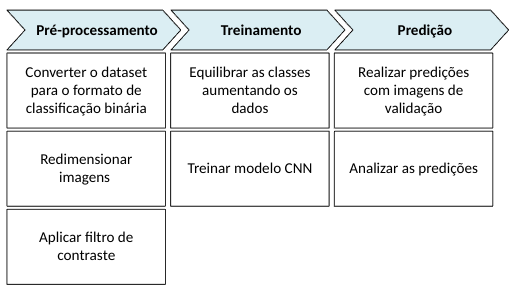
\includegraphics[width=0.5\textwidth]{images/metodologia.png}}
    \caption{Example of a figure caption.}
    \label{fig:metodologia}
\end{figure}

\subsection{Pré-processamento}\label{AA}

O conjunto de dados fornecido por \cite{Deitsch2021} contêm 2.426 imagens de
eletroluminescência obtidas de células de painéis
solares reais. Cada imagem no dataset contém uma célula individual de silício
policristalino ou monocristalino. Todas as imagens foram rotuladas por um
especialista,
indicando a probabilidade da célula estar danificada.
Durante a etapa de pré-processamento, os valores de
probabilidade são convertidos em uma classe binária, classificando as imagens
como "Defeituosa" ou "Não Defeituosa". Nesse processo imagens rotuladas com
probabilidade acima de 60\% são categorizadas como "Defeituosa", enquanto
aquelas com uma probabilidade igual ou inferior a este limiar são rotuladas
como "Não Defeituosa".

As imagens foram redimensionadas para
224x224 pixels. Em seguida, foi aplicado um filtro de equalização de histograma
usando a função \textit{createCLAHE} da biblioteca OpenCV [REFER], a qual
ajusta o contraste da imagem de maneira adaptativa, limitando o aumento de
contraste para evitar a ampliação do ruído.

Na Fig.\ref{fig:amostras-dataset} são apresentadas quatro amostras do dataset
reclassificado.

\begin{figure}[htbp]
    \centering
    \begin{tabular}{cc}
        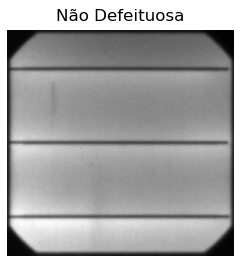
\includegraphics[width=0.20\textwidth]{images/mono-no-defect.png} &
        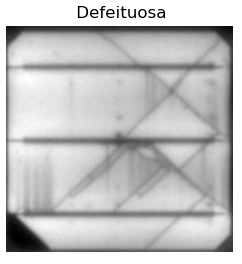
\includegraphics[width=0.20\textwidth]{images/mono-defect.png}
        \\
        \textbf{2 (a)}                                                    &
        \textbf{2 (b)}                                                      \\
        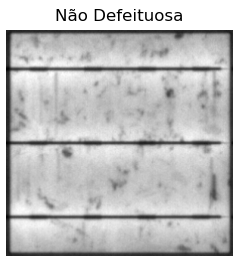
\includegraphics[width=0.20\textwidth]{images/poly-no-defect.png} &
        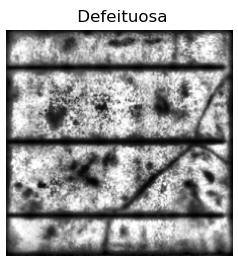
\includegraphics[width=0.20\textwidth]{images/poly-defect.png}
        \\
        \textbf{2 (c)}                                                    &
        \textbf{2 (d)}                                                      \\
    \end{tabular}
    \caption{Amostras do dataset de células fotovoltaicas: 2(a) monocristalina
        sem defeito, 2(b) monocristalina com defeito, 2(c) policristalina sem
        defeito,
        2(d) policristalina com defeito. \cite{Deitsch2021}}
    \label{fig:amostras-dataset}
\end{figure}

\subsection{Treinamento}\label{AA}

Mesmo após a etapa de pré-processamento, a disposição das classes no dataset
estava desbalanceada, pois as células com defeitos representavam apenas
31.3\% do total de imagens. Para contornar este problema, foi empregado
o método de aumento de dados no conjunto de imagens classificadas como
"Defeituosa", com o auxílio da biblioteca. O gráfico na
Fig.\ref{fig:dataset-overview} apresenta a disposição final do dataset de
referência.

\begin{figure}[htbp]

    \centerline{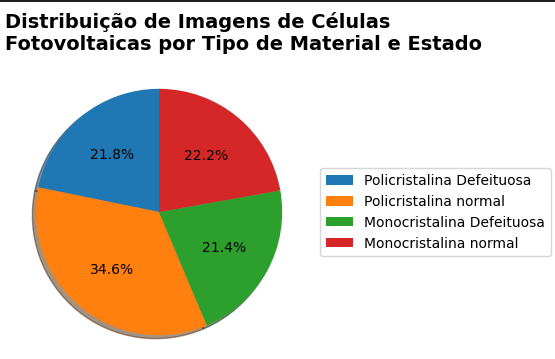
\includegraphics[width=0.5\textwidth]{images/dataset-overview.png}}
    \caption{Distribuição do dataset de referência quanto ao tipo de célula
        fotovoltaica e o estado.}
    \label{fig:dataset-overview}
\end{figure}

O dataset processado foi dividido de forma randômica em dois conjuntos, um de
treinamento
com 75\% (2382 imagens) e outro de teste com 24\% (779 imagens). Os
hiperparâmetros do modelo foram definidos empiricamente, com base em
experimentos e ajustes realizados durante o processo de desenvolvimento.
\ref{tab:hiperparametros}.

\begin{table}[h!]
    \caption{Hiperparâmetros do modelo CNN(24)}
    \centering
    \begin{tabular}{|c|c|}
        \hline
        \textbf{Parâmetro}   & \textbf{Valor}       \\ \hline
        Tamanho do kernel    & 3x3                  \\ \hline
        Taxa de aprendizagem & 0.001                \\ \hline
        Number of Epochs     & 100                  \\ \hline
        Tamanho do lote      & 14                   \\ \hline
        Função de perda      & binary\_crossentropy \\ \hline
        Otimizador           & Adam                 \\ \hline
    \end{tabular}
    \label{tab:hiperparametros}
\end{table}

\subsection{Predição}\label{AA}

Na última etapa, foram realizadas predições com o modelo treinado utilizando
um conjunto de 15 imagens. Além disso, avaliou-se a eficácia do modelo proposto
por meio de métricas de avaliação, como acurácia, perda e .

\section{Resultados}

A acurácia do modelo proposto com o conjunto de teste foi de 72.76\%, e perda de 60.45\%. A Fig \ref{fig:training-accuracy} apresenta a curva de acurácia do modelo
durante
o treinamento, enquanto a Fig \ref{fig:training-loss} mostra a curva de função
de perda.
A Fig \ref{fig:confusion-matrix} apresenta a matriz de confusão do modelo,
enfatizando que o modelo identificou corretamente XX\% das células defeituosas.

\begin{figure}[htbp]

    \centerline{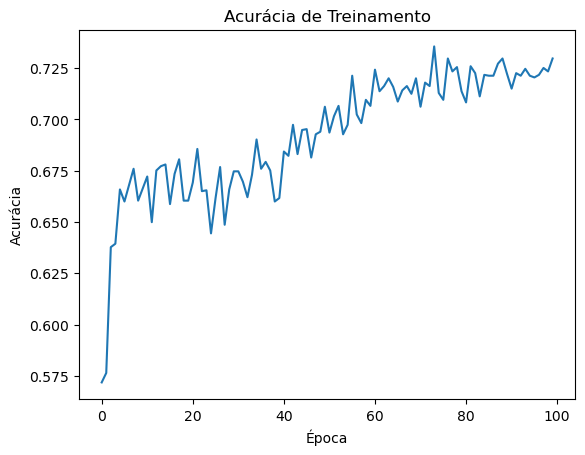
\includegraphics[width=0.4\textwidth]{images/training-accuracy.png}}
    \caption{Acurácia do treinamento ao longo das épocas.}
    \label{fig:training-accuracy}
\end{figure}

\begin{figure}[htbp]

    \centerline{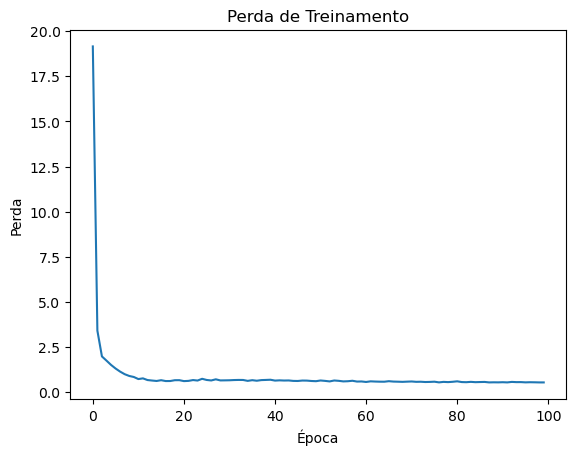
\includegraphics[width=0.4\textwidth]{images/training-loss.png}}
    \caption{Perda do treinamento ao longo das épocas.}
    \label{fig:training-loss}
\end{figure}

\begin{figure}[htbp]

    \centerline{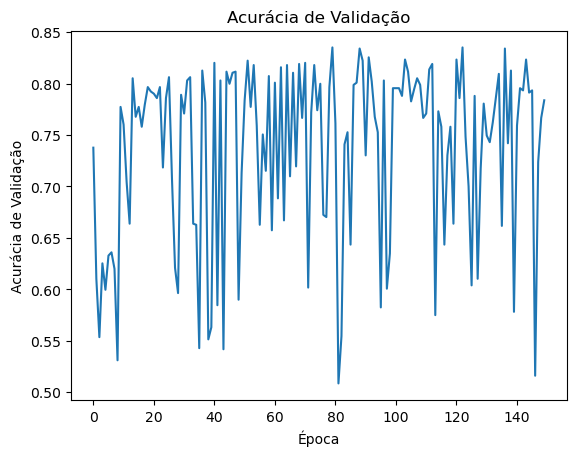
\includegraphics[width=0.4\textwidth]{images/validation-accuracy.png}}
    \caption{Acurácia da validação ao longo das épocas.}
    \label{fig:validation-accuracy}
\end{figure}

\begin{figure}[htbp]

    \centerline{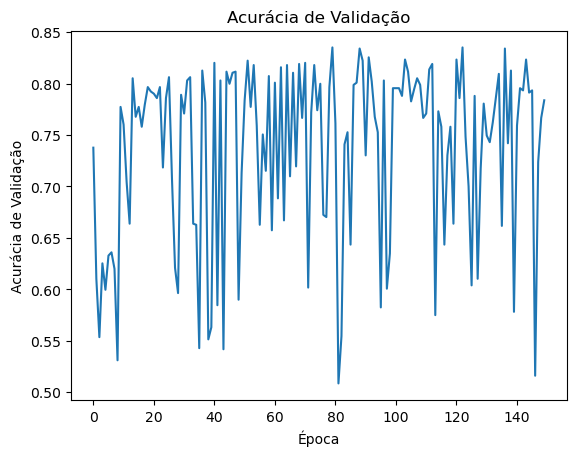
\includegraphics[width=0.4\textwidth]{images/validation-accuracy.png}}
    \caption{Matriz de confusão para o conjunto de teste.}
    \label{fig:confusion-matrix}
\end{figure}
\section{Conclusão}

Com base nos resultados apresentados, conclui-se que a rede neural proposta
neste
trabalho não obteve um desempenho satisfatório na classificação de células
fotovoltaicas defeituosas. O modelo se mostrou ineficaz na identificação de
defeitos nas imagens de eletroluminescência, com uma acurácia de XX\%. Durante
a etapa de predição observou-se que o modelo apresentou dificuldade
principalmente em classificar principalmente células de silício policristalino
DADO. Acredita-se que a textura natural observada nas imagens de
eletroluminescência de células policristalinas tenha dificultado a
identificação de defeitos pelo modelo.

Para trabalhos futuros, sugere-se o uso da técnica transferência de
aprendizagem para melhorar o desempenho do modelo. A técnica de transferência
de aprendizagem consiste em utilizar um modelo pré-treinado em um conjunto de
dados maior e mais diversificado, como por exemplo o \textit{ImageNet}.

\bibliographystyle{IEEEtran}
\bibliography{references}
\end{document}
